\chapter{Server Side}
\paragraph{}
This chapter discusses the server side of WebSlicer in detail. 
Included with this is some necessary background about JavaEE and some of its functions.

\begin{figure}[!ht]
  \centering
  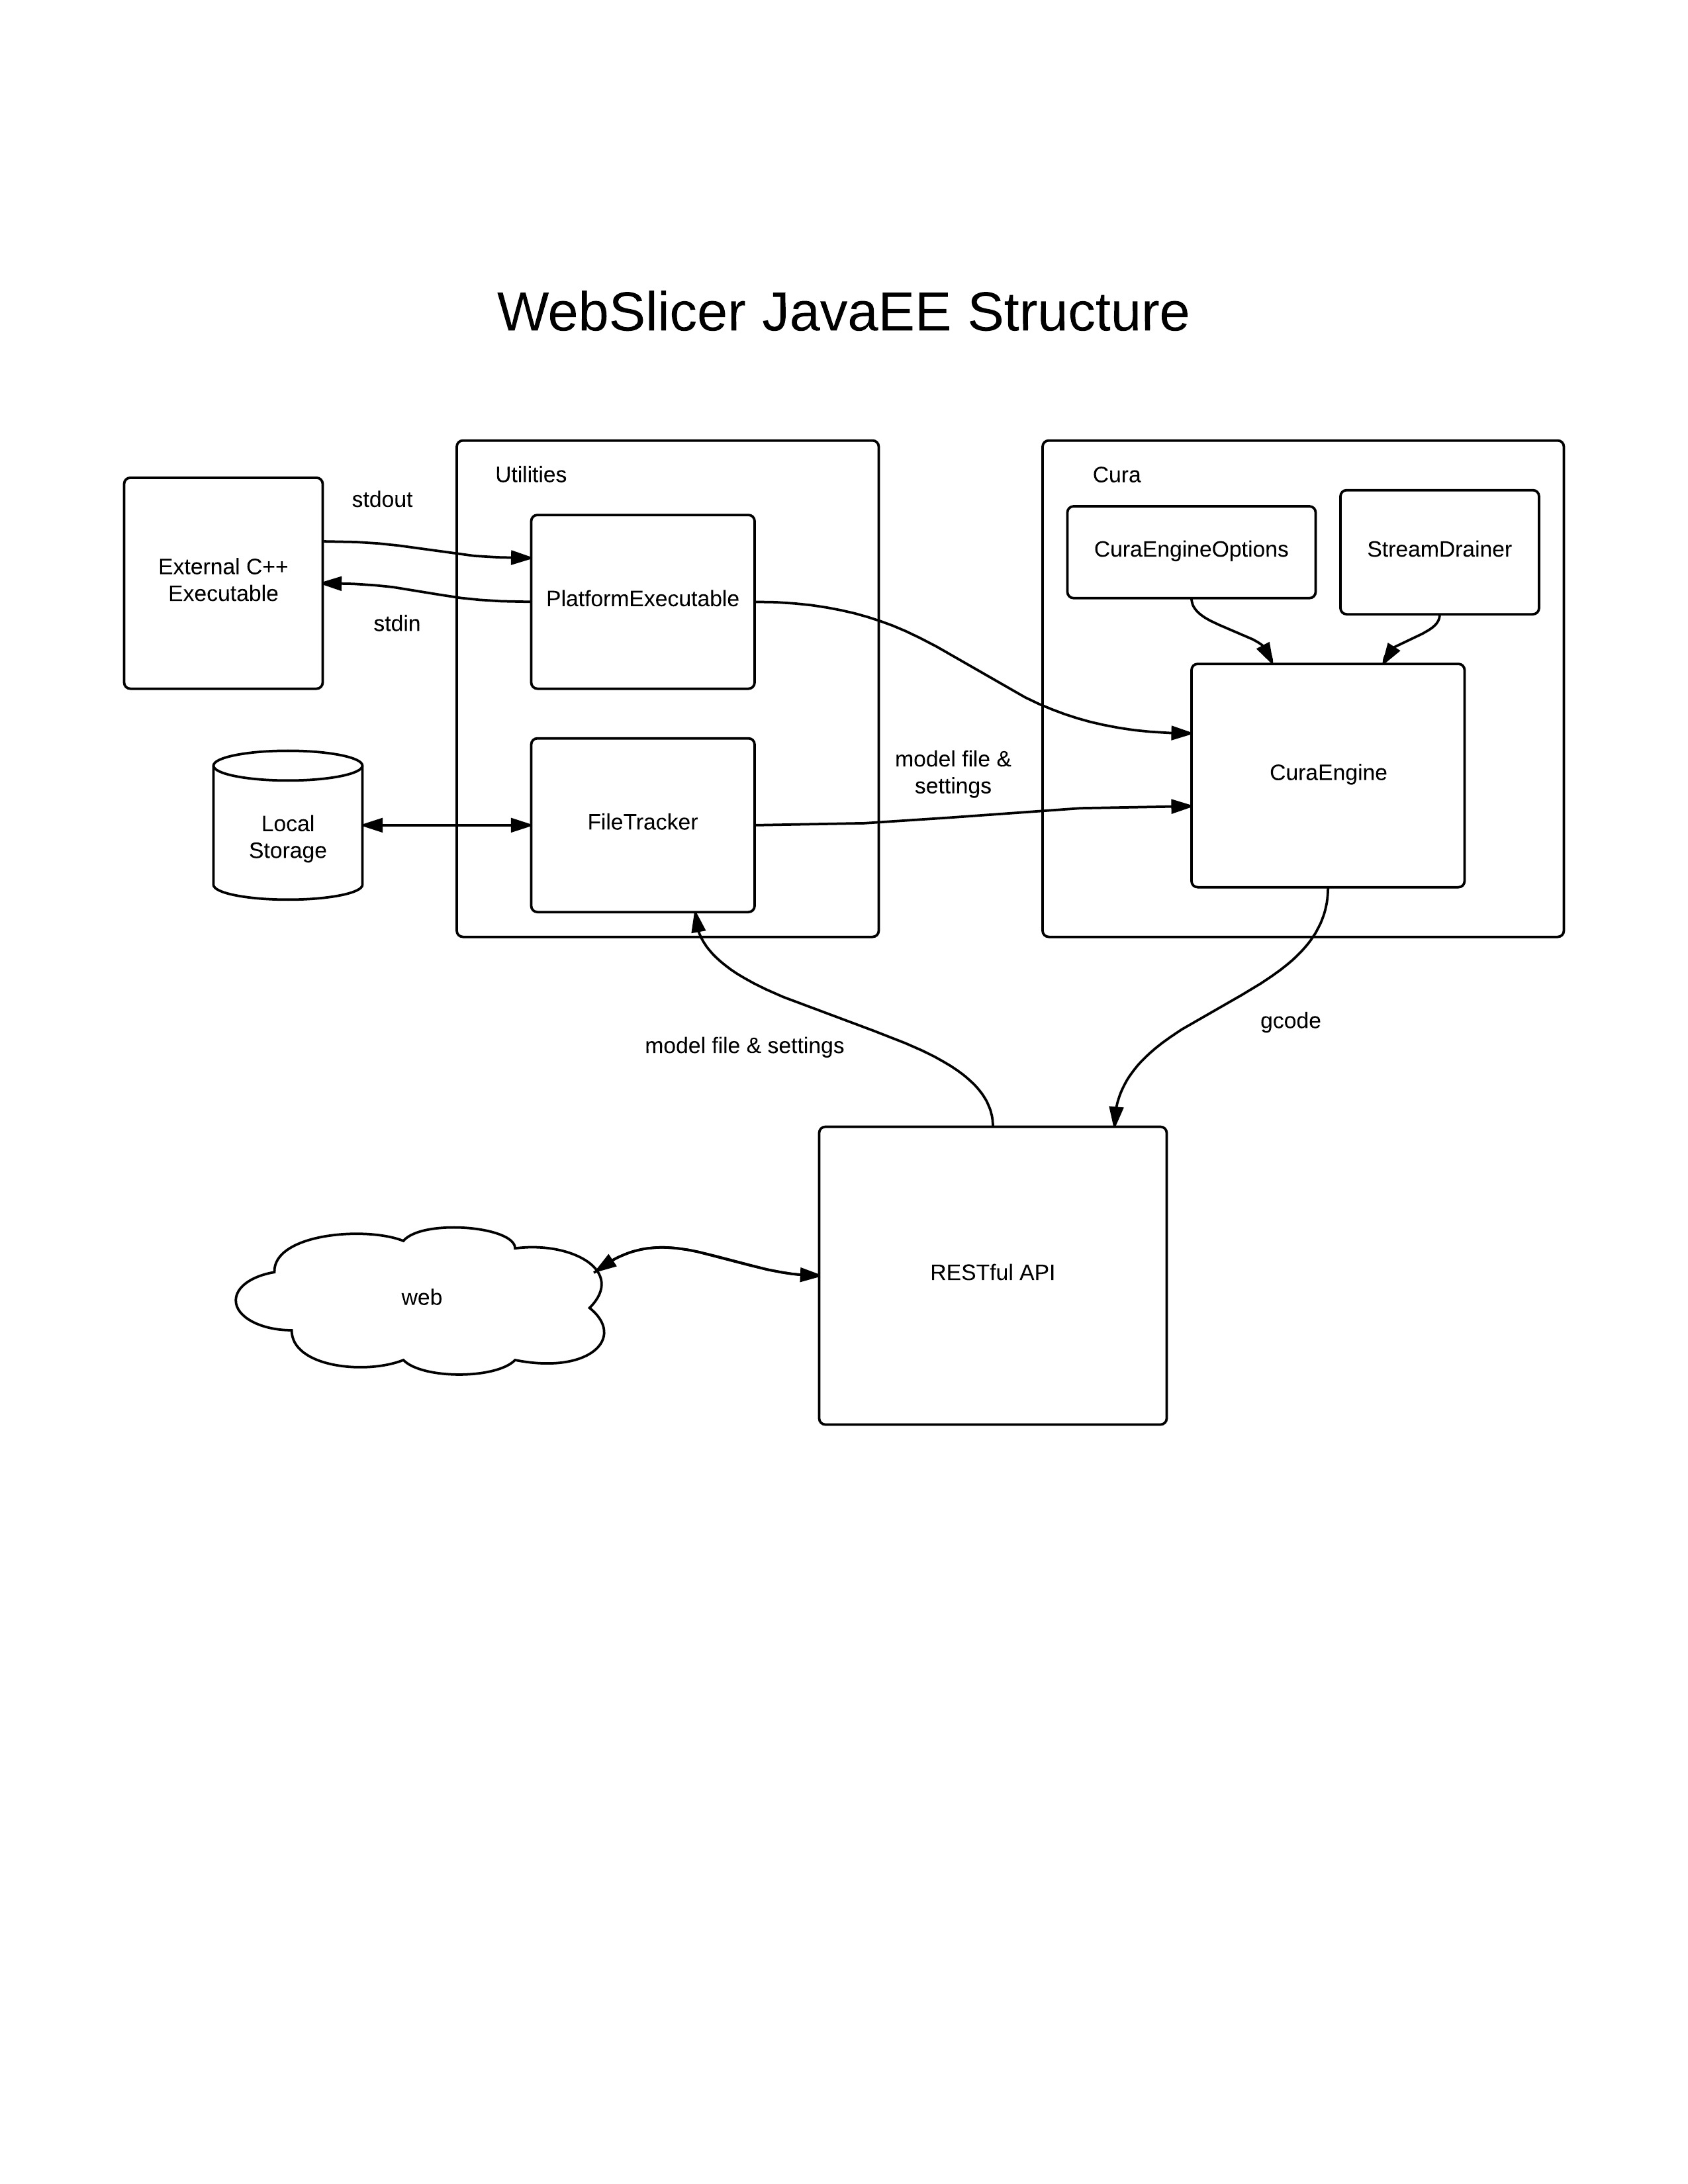
\includegraphics[width=\linewidth]{diagrams/Server-Side-Structure}
  \caption{The structure of the server side of WebSlicer}
  \label{fig:server-side-structure}
\end{figure}

\section{JavaEE Structure}
\paragraph{}
The server side of WebSlicer was written in JavaEE, the structure for which is shown in Figure \ref{fig:server-side-structure}.
JavaEE was the optimal choice for this application, as it allowed for the easiest deployment and was also the easiest to scale \citep{pilgrim-2013}.
Additionally, JavaEE has a excellent code packaging mechanism for web and non web based applications alike.
The web container which is in use for this application exposes a RESTful API on a privately hosted server.

\paragraph{}
To further simplify the development process, Maven was also used.
Maven is a build tool for Java and has support for deploying complex applications such as those in JavaEE \citep{massol-2005}.
Thus, when a build was completed, it was automatically deployed and ready for testing.

\section{ProcessBuilder}
\paragraph{}
At the core of the server side application is an executable called CuraEngine. 
It is the main executable which is compiled from the open source slicing platform Cura which is written in C++. 
This presented a problem, as all of the server side code in this application is written in Java. 
ProcessBuilder was the solution to this problem as it is capable of redirecting the input and output streams of a local executable process into the Java server application.
CuraEngine from Figure \ref{fig:server-side-structure} uses a ProcessBuilder and the PlatformExecutable to create a runnable Java method that is capable of executing like a C++ executable.
CuraOptions feeds the CuraEngine class with all of the parameters that it needs from the API.
It gathers the path to the appropriate settings file and includes all of the parameters needed to run the CuraEngine executable.

% running CuraEngine from the command line example
\lstsetconsole
\begin{lstlisting}[language=sh, label={lst:curaengine-executable}, caption=An example of running CuraEngine C++ executable directly from the command line.]
CuraEngine slice -v -j {settings.json} -g -e -o {output.gcode} -l {model-file.stl}
\end{lstlisting}

\paragraph{}
An example of running the CuraEngine C++ executable from the command line is shown in Listing \ref{lst:curaengine-executable}.
When the ProcessBuilder class of WebSlicer receives a slice command from the API it gathers the arguments listed in brackets and sends them to PlatformExecutable.
PlatformExecutable then spawns a native process and pipes its input and output streams into the respective Java streams.
In the meantime, StreamDrainer spawns a new thread and waits for the output stream that was created by PlatformExecutable.
StreamDrainer's task is to take the unneeded output from stdout and pipe it into a log file for debugging.

\paragraph{}
After CuraEngine has finished slicing the current file and PlatformExecutable has returned the REST API, which has been waiting, it unblocks and starts reading the output gcode file.
This file is then packaged and sent back to the client as the response of the ``/slice/\{clientId\}/\{modelId\}'' command as shown in Table \ref{tab:restapi}.

\section{REST API}
% my REST API and the reason that I structured it the way I did
\begin{table}[h]
  \centering
    \begin{tabularx}{\textwidth}{ |l|l|X| }
      \hline
      Type & Address & Description \\ \hline
      \hline
      GET & /ping & A simple ping endpoint used for testing. \\ \hline
      POST & /setupClient & Sets aside all needed files for a new client and return its unique ID. \\ \hline
      POST & /importStl/\{clientId\} & Takes a MIME type file stream and imports the file to the clientId specified in the URL. It also returns a unique identifier for the file. \\ \hline
      POST & /importSettings/\{clientId\} & Similar to importStl this endpoint takes a settings JSON file and imports it to the specified clientId \\ \hline
      POST & /slice/\{clientId\}/\{modelId\} & This is the main slice function of the API. It combines all of the parameters specified by the calls before and returns a gcode file to the user. \\ \hline
      POST & /testSlice & A test endpoint that requires no parameters and simply returns some arbitrary gcode to the user. \\ \hline
      GET & /getFiles/\{clientId\} & Returns all the model file names and their tracking ID's that are associated with a clientId. \\ \hline
    \end{tabularx}
  \caption{Documentation of all exposed endpoints of the RESTful API}
  \label{tab:restapi}
\end{table}

\paragraph{}
The goal of the client is to satisfy all the requirements needed to run the ``/slice'' command from Table \ref{tab:restapi}.
A typical call pattern to the API in begins with creating a user if one does not already exist.
Creating a new user requires calling ``/setupClient'' and recording the returned unique user identifier.
Using the recorded unique identifier the client must then upload a model file and settings file to the corresponding ``/importStl'' and ``/importSettings'' functions.
This returns unique identifier strings for all settings and model files that the client uploads to the server.
Finally, to run a slice, the client takes all acquired unique identifiers and places them into the call to ``/slice'' as shown in Table \ref{tab:restapi}.
Upon successful completion of all aforementioned calls the user will be returned a G-code file in raw textual form.

% add typical call pattern here

\section{Key Challenges}
\subsection{ProcessBuilder Deadlock}
\begin{figure}[!ht]
  \centering
  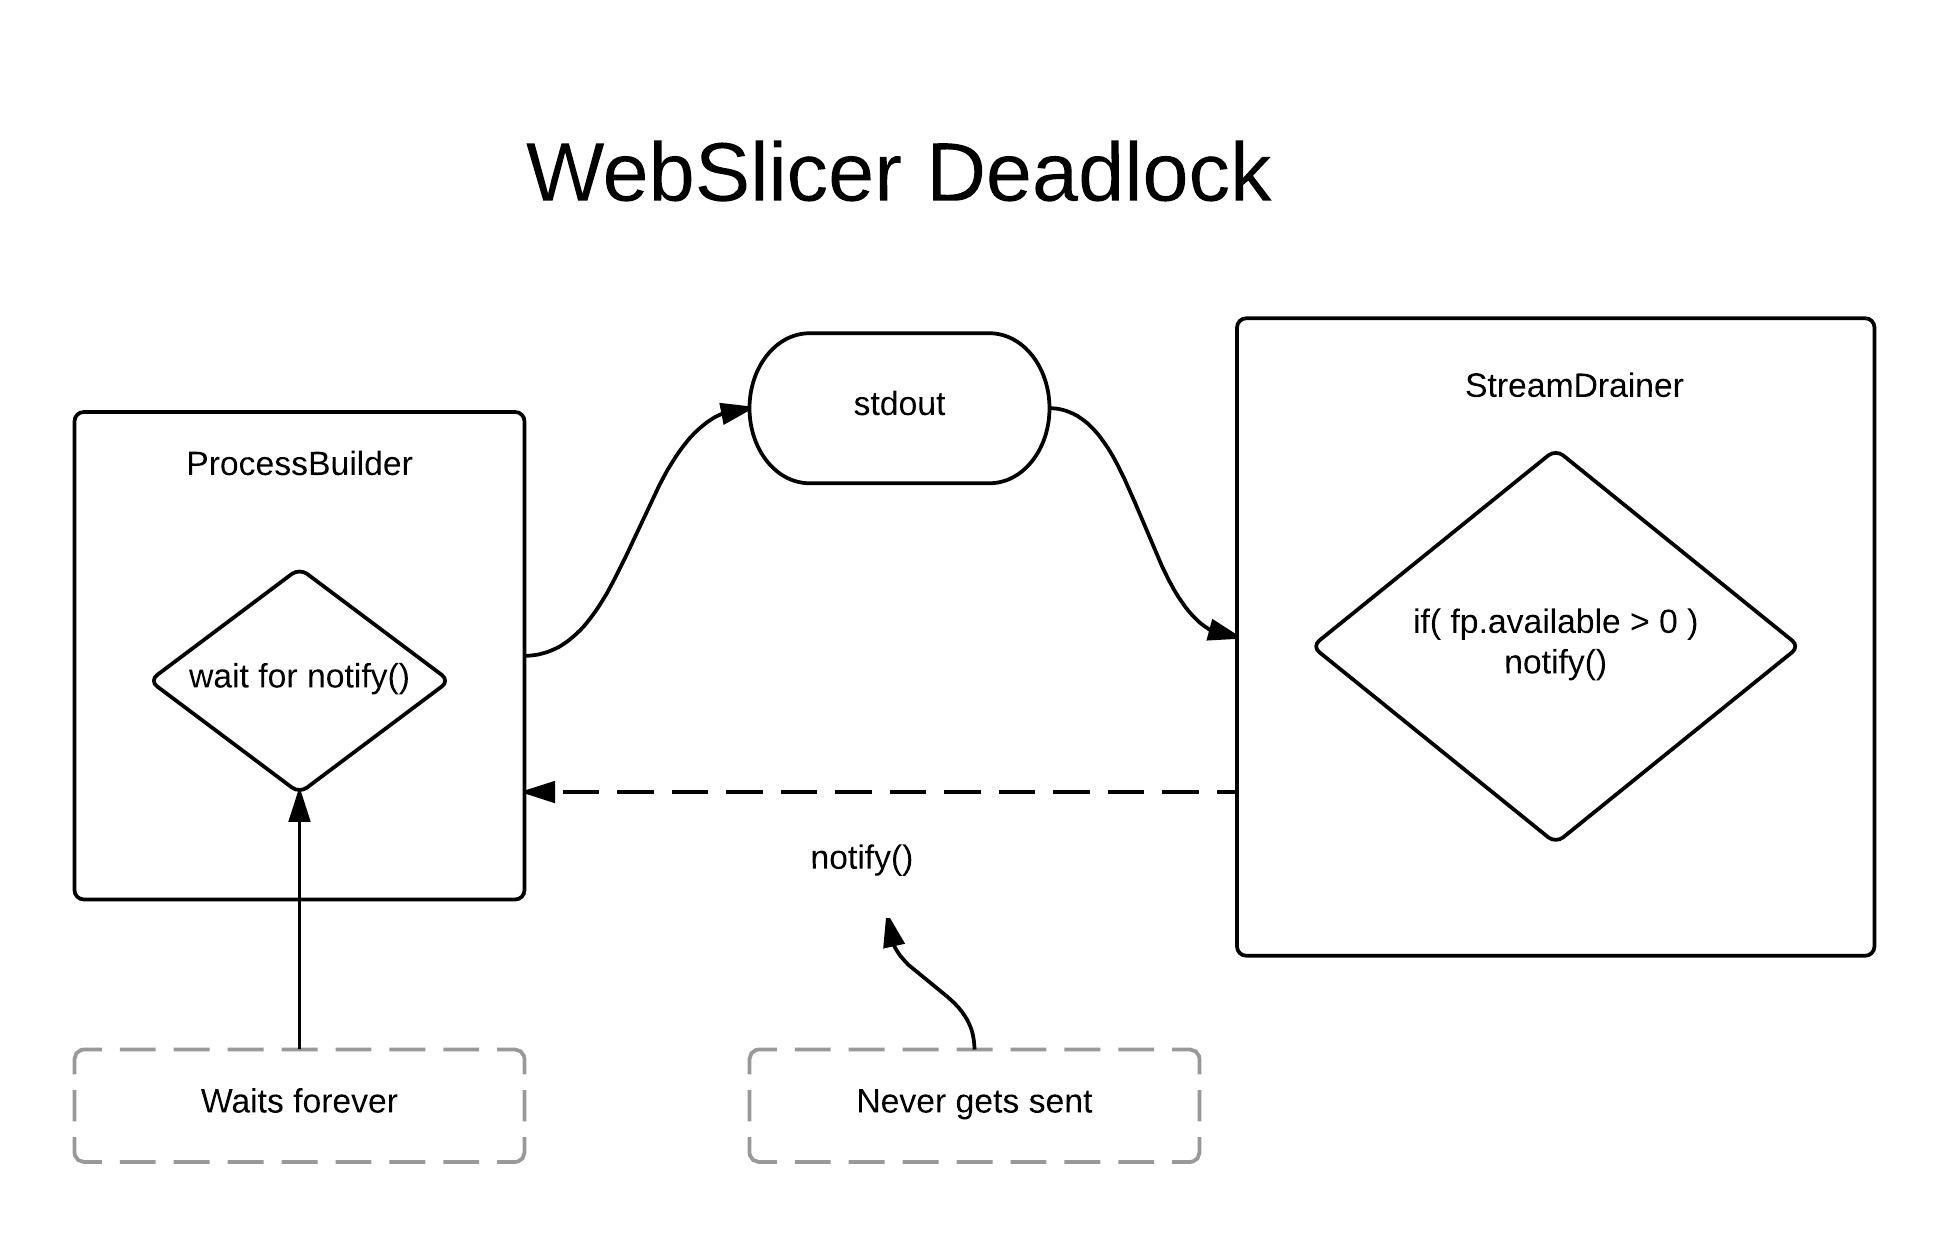
\includegraphics[width=\linewidth]{diagrams/Deadlock-Diagram}
  \caption{Diagram of a deadlock issue that took weeks to resolve}
  \label{fig:deadlock-diagram}
\end{figure}
\paragraph{}
One considerable bug encountered while developing this project was a thread deadlock issue. 
The server side code uses Java's ProcessBuilder, which builds a system native call to an executable and then pipes the input and output into the corresponding pipes of Java's stdio as shown in Figure \ref{fig:deadlock-diagram}.
This is suitable for small platform executables with limited I/O, but can become problematic when complex native calls such as CuraEngine are used.

\paragraph{}
ProcessBuilder executes its normal writes to stdout and the drainer pipes them into a file; however, the drainer must wait for a file pointer using the fp.available() function. 
This is a non-blocking function that only estimates the buffer size that it has for the file. 
The check for file pointer availability was determining whether this function returned something greater than 0 as an estimate before notifying the ProcessBuilder that it was ready;
however, the buffer size would often start as zero before allocation and, as this check was not part of a loop, it would stay stuck forever as the notify was missed.

\paragraph{}
This problem was solved by using the correct blocking file pointer available check. 
Occasionally, the buffer size was larger than 0 and the application ran suitably but, with some models, it would consistently fail, as the buffer had not been allocated yet.
This solution is seemingly obvious yet it took many days to find and correct because the application did not fail consistently.

\subsection{FileTracker Revamp}
\paragraph{}
The first iteration of FileTracker was crude and not well planned out. 
It tracked two hash maps: one for model files and the other for settings files with no mind for the client who required access to those files. 
This worked for testing, but incurred many pitfalls including the inability to reuse files that already existed. 
As soon as the client closed their session, those files were lost, which is a major inefficiency.

\paragraph{}
The fdmprinter.json file within the unique client folder is symbolically linked to the fdmprinter.json file within the common folder. 
The CuraEngine executable requires that all of the settings files rest within the same directory when performing a slice as shown in Listing \ref{lst:file-structure}.
Unfortunately, this leaves the potential result of having this file copied for many clients. 
Thus, symbolically linking the file to the rescue.

\paragraph{}
The output.gcode and settings.json files are dynamically overwritten for every iteration so their existence here is only for the sake of running CuraEngine through file arguments.
The user has no access to these files and is only able to obtain their content through the web interface, which parses in and out of files.

% listing of the file structure that FileTracker creates
\lstsetxml
\begin{lstlisting}[language=XML, label={lst:file-structure}, caption=WebSlicer's underlying file structure supported by FileTracker.]
webslicer/
- b1a2a69e-5893-4d7c-aa1f-d639fa3b4ed1/
  - fdmprinter.json -> /tmp/webslicer/common/fdmprinter.json
  - models/
     - balanced_die_version_2.stl
     - raldrich_planetary.stl
  - output.gcode
  - settings.json
- common/
  - fdmprinter.json
  - presets/
    - prusa_i3.json
    - ultimaker2.json
\end{lstlisting}

\section{Future Improvements}
\paragraph{}
Currently, FileTracker does not take advantage of the presets within the ``common/presets/'' folder as described by Listing \ref{lst:file-structure}. 
These files contain the default settings for the corresponding printer, which are the ultimaker2 and a basic configuration of a prusa i3 variant. 
Optimally, the user would select from one of these starting presets and then modify and save their own.
This would allow users an optimal starting point while lowering the amount of starting knowledge and increasing the usability of WebSlicer.

\paragraph{}
This new file structure also allowed for an easy client index. 
In the future, the unique folder ID will become the client's identification number, which will be attached to their login. 
Additionally, simplifying the login process with Google's OAuth 2.0 system was also planned.

\section{Issues \& Known Bugs}
\paragraph{}
Currently there is no way for the server to import existing user files into its structure.
Thus, when the server is restarted for any reason, the supporting file structure with all user files is lost.
Resolving this is just a matter of writing an initial import function that indexes all of the existing files.
It was removed from the initial version due to time constraints.
